\begin{figure}[H]
\begin{center}
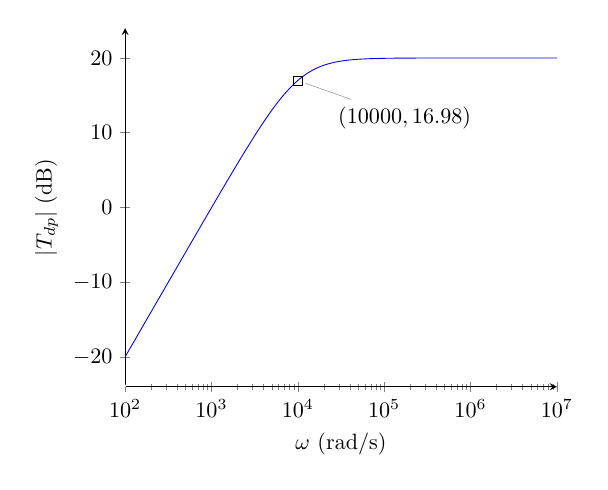
\begin{tikzpicture} [scale=0.8]
\begin{semilogxaxis}[
    axis lines = left,
    xlabel = {$\omega$ (rad/s)},
    ylabel = {$|T_{dp}|$ (dB)}
]
\addplot [
    domain=100:1000000, 
    samples=100, 
    color=white,
]
{24*log10(10*x/sqrt(x^2+(10000)^2))};
\addplot [
    domain=100:10000000, 
    samples=100, 
    color=blue,
]
{20*log10(10*x/sqrt(x^2+(10000)^2))};
\addplot[mark=square] coordinates {(10000,16.98)} node[pin=-30:{$(10000,16.98)$}]{};
\end{semilogxaxis}
\end{tikzpicture}
\hspace{1cm}
\begin{tikzpicture} [scale=0.8]
\begin{semilogxaxis}[
    axis lines = left,
    xlabel = {$\omega$ (rad/s)},
    ylabel = {$\angle T_{dp} $ (°)},
    xtick={10,100,1000,10000,100000,1000000,10000000},
    ytick={-180, -135, -90},
]
\addplot [
    domain=10:10000000, 
    samples=100, 
    color=blue
]
{-180+atan(10000/x))};
\addplot[mark=square] coordinates {(10000,-135)} node[pin=220:{$(10000,135)$}]{};
\addplot [
    domain=10:10000000, 
    samples=100, 
    color=white
]
{-90};
\addplot [
    domain=10:10000000, 
    samples=100, 
    color=white
]
{-180};
\end{semilogxaxis}
\end{tikzpicture}
\end{center}
\caption{Curvas de bode teóricas da função de transferência do derivador.}
\label{bode:2} 
\end{figure}